\subsection*{Optimized Detector Array}\addcontentsline{toc}{subsection}{Optimized Detector Array}
%detectordetails.1.0.tex

\begin{wrapfigure}[26]{r}{3in}
\vspace{-3\baselineskip}
\centerline{\includegraphics[width=\linewidth]{applsci-08-01039-g005-550.eps}}
\centerline{\includegraphics[width=\linewidth]{applsci-08-01039-g006-550.eps}}
\vspace{-1\baselineskip}
\caption{\label{fig::thomasfigs}Reproduced from Ref.~\cite{Feurer2018}. (upper) X-ray pulse retrieval error versus \% energy resolution.  
(lower) Retrieval error versus angular sampling.}
\end{wrapfigure}

The technical requirements that enable pulse retrievals for accurate reconstruction are not trivial to achieve.
Pulse-to-pulse variations at an FEL require single-shot measurements much like the velocity map imaging (VMI) \cite{VrakkingRSI} extension of attosecond angular streaking \cite{attoclockVMI2013}.
Although we have explored such a single-shot VMI solution for 120~Hz operation \cite{Siqi2018}, its requirement of a two-dimensional area detector precludes its use for the high repetition rates expected. 
Furthermore, the single resolution window of the VMI precludes its use for the kinds of novel multi-color pulses we have come to expect from LCLS \cite{Lutman13_twocolor,Marinelli13_twocolor,Marinelli2015,Lutman2016,LutmanFreshSlice2016}.
We are therefore designing toward a single-shot diagnostic that reports the full temporal intensity, wavelength, and polarization distribution also with attosecond scale resolution and at the highest repetition rates up to 1~MHz.  
We further require a two-fold over sampling in the angular dimension in order to fully characterize even multi-pulses (Fig.~\ref{fig::2color2polResults}) \cite{Lutman2016,LutmanFreshSlice2016}.
Modeled after the original so called ``Cookie Box'' design of Jens Viefhaus, we propose a main chamber that accepts micro-channel plate based electron detectors in a 16-fold symmetric angular array.

Preliminary results of Ref.~\cite{Nick2018} were based on 1~eV eTOF spectrometer resolution when working in the required single-shot current mode (Viefhaus points in Fig.~\ref{fig::detectorcompare}.
We note that used in counting mode as at a synchrotron, higher resolution can be achieved by electron event edge detection, but the FEL use case requires a direct spectral readout with the MCP electronics run in ``current'' mode with the voltage waveform being digitized as a single shot spectrum.
This sets the resolution not by how well one can locate the center of the impulse response waveform, but rather the actual width of that impulse response waveform.
This motivates us to design for the sharpest achievable response from the MCP assembly and that we digitize that waveform with appropriately high sampling over a sufficiently long temporal span.
The current target of 400~ps FWHM for the MCP response then pushes us to design for at least 5~GSps digitizer sampling over at least a 200~ns long window.

Although the final decision on retrieval algorithm is a subject of active research, we use so called ``Attoclock Ptychography'' \cite{Feurer2018} to inform our specifications for spectral and angular resolution.
From Fig.~\ref{fig::thomasfigs}(upper) we can see that the energy resolution for the streaked photoelectrons should ideally be in the sub~0.25\% range.
The fine tuning of the sorts of novel FEL modes that allow for attosecond \cite{xLEAP} and two-color \cite{LutmanFreshSlice2016} FEL experiments typically also require 0.25~eV resolution \cite{AlbertoPrivate}.
We are therefore targeting 0.5~m long eTOF spectrometers which we expect to give an energy resolution of 0.25~eV at up to 100~eV electron kinetic energy above the retardation voltage, based on an estimated comparison of existing detectors (points) to the simulations (line segment) shown in Fig.~\ref{fig::detectorcompare}.

\begin{wrapfigure}[17]{l}{3in}
\centerline{\includegraphics[width=\linewidth]{nphoton.2016.79.2color2pol.eps}}
\caption{\label{fig::2color2polResults}Two-polarization, two color, pulse pair demonstration using the original CookieBox, reproduced from Ref.~\cite{Lutman2016}}
\end{wrapfigure}
The resolution in pulse reconstruction depends also on the number of angular sample points per optical cycle.
In Fig.~\ref{fig::thomasfigs}(lower) we see a clear prescription that the angular streaking pattern should be sampled at least along 6--8 angular sample points.
The diminishing returns for adding more detector assemblies drives the design to 16 angles, providing a two-fold over-sampling of the angular dimension for the sake of our two-color aspirations.
Furthermore, by shifting the dressing laser frequency toward the near-infrared we can further improve the temporal resolution.
Based on Refs.~\cite{lcls2_opportunities,Cederbaum2008,Biggs2012,Mukamel2013} we expect that much of the x-ray pulse characterization needs will lie in the sub-10 fs regime.
We propose therefore to shift to a 2-3~$\mu$m wavelength for the streaking laser to improve the temporal resolution while still preserving an appropriate window for pulse shape retrieval.
The shorter wavelengths also typically improve the fractional bandwidth for a more robust carrier shape, though stable and ultrashort THz \cite{Matthias2008,MatthiasReview2011,Hauri2011} and mid infrared \cite{Sell2008,Cavalleri2010} are active research topics at SLAC and indeed will aid the retrieval of long duration shaped x-ray pulses. 
Nevertheless, a change to short wavelength should take our initial demonstration of 500 attosecond resolution for a 10~$\mu$m, 33~fs optical cycle, angular streaking field to an expected 150 attoseconds resolution for a 3 $\mu$m field --- 11 fs optical cycle.
Figure~\ref{fig::jamessim} shows a 4~$\mu$m wavelength simulation of two xFEL pulses that are separated by only 4~fs.
By pushing further down to a 1~$\mu$m streaking field, we could expect to achieve temporal resolutions competitive with laser-based HHG state-of-the-art \cite{Zenghu2017,HJWorner2017}.

\begin{wrapfigure}[16]{r}{3.5in}
\vspace{-1.5\baselineskip}
%\centerline{\includegraphics[width=\linewidth]{plotting.tofs.compare.forproposal.eps}}
\centerline{\includegraphics[width=\linewidth]{plotting.tofs.compare.forproposal.new.eps}}
\vspace{-0.5\baselineskip}
\caption{\label{fig::detectorcompare}Detector resolution versus length comparison. }
\end{wrapfigure}

When diagnosing closely separated double pulses, the angular acceptance of the electron spectrometers are a principle concern \cite{Worner2018}.
We plan to optimize this angular acceptance such that we relax slightly the collection efficiency of each detector for the sake of preserving the energy resolution.
We were able to reduce the sample density by 10-fold in Ref.~\cite{Nick2018} to avoid the onset of space-charge blurring of the streaking resolution.
We expect that we can sacrifice a factor of 6 in signal in order to relax the angular collection of the eTOFs also by partially compensating for this loss by using new funnel-pore microchannel plates \cite{funnelMCPcompare2018}.


We are designing for a novel configuration whereby individual detectors in the eTOF array can have vastly different retardation voltages.
Motivated by the great progress in multi-color FEL modes \cite{Lutman13_twocolor,Marinelli13_twocolor,Allaria2014,Marinelli2015,Prince2016,Lutman2016,Marinelli2016,LutmanFreshSlice2016}, we will capitalize on the two-fold over sampling in the angular dimension to accommodate extreme color separations between multi-pulses.
Figure~\ref{fig::sxu_K} shows that the soft x-ray undulator (SXU) for LCLS-II will be capable of K values from 2 to 5 that could provide two-color pulses with one pulse below the carbon edge and the other above the oxygen edge.
We plan for tests of such a novel mode by demonstrating interleaved retardations used to measure the carbon and the oxygen Auger electron spectra simultaneously with high resolution as early as spring 2020.



\subsection*{Real time analysis}\addcontentsline{toc}{subsection}{Real time analysis}
%realtimeanalysis.0.0.tex
\begin{wrapfigure}[20]{r}{3.5in}
\vspace{-0.5\baselineskip}
\centerline{\includegraphics[trim={0 0 0 0pt},width=\linewidth]{jamessim.eps}}
\vspace{-0.5\baselineskip}
\caption{\label{fig::jamessim}Simulation of two attosecond x-ray pulses separated by 4~fs dressed by a 4~$\mu$m streaking field, courtesy J.~Cryan.}
\end{wrapfigure}


Given the MHz scale repetition rate of Table~\ref{lcls2specs} for LCLS-II, a measure-and-sort method that required every XFEL shot be recorded would increase the data load from the 10 TB/day of today to 100 PB/day.
Such a load would require an enormous cost for developing the ultra-high duty-cycle area detectors and the corresponding network and storage infrastructure. 
If instead one could use real-time information about the x-ray pulse shape, then one could veto events where the pulse characteristics were not amenable to the physics being measured.
Furthermore, one could allow for on-board histogram updates in a memory buffer that could collate the real-time sorted results prior to network transfer.
Such a vision fuels our strong motivation to not only provide high repetition rate veto, but also event rate, low-latency sorting triggers.

The on-board analysis of the data is a challenging bottleneck in the angular streaking scheme.
The raw data in angular streaking is the digitized waveform spanning about 500~ns of record length with a sample frequency of ideally about 10GS/s, one waveform for each of the 16 detectors.
Transferring and writing this data would require nearly 160~GBps steady-state continuous feed.
We therefore require that the analysis occur ideally directly in combination with the digitization.
All together though, this analysis would be comparable to analyzing one $256\times256$ 10 bit deep image every microsecond.

Detailed in Ref.~\cite{Nick2018}, we iteratively account for intensity in the polar representation of the angular photo-electron spectrum.
This so called ``PacMan'' routine as well as a similar methods \cite{Thomas2015,Siqi2018,Worner2018} and certainly ``Attoclock Ptychography'' \cite{Feurer2018} are computationally expensive and are not likely to allow MHz or even 100 kHz data throughput.
They certainly will not achieve the desired microsecond scale latency for providing sort and veto triggers.
We therefore plan to reserve such computationally expensive methods for the generation of so-called ``ground truth'' x-ray pulse shapes for a sub-set of full fidelity raw data.

We plan to use the ground truth set for training and validating a low-latency inference matrix solution that could be implemented as a series of FPGA-based on-board matrix multiplications.
Only very small data of the retrieved pulse would be transferred to remote data recording nodes along with intermittent high fidelity shots for continually populating the validation and re-training sets.
We will use simulations of angular streaking from expected FEL pulses, together with the detector array simulations used for the design modelling, to iterate on the detector hardware configurations and the analysis pipeline from electronics to inference output.
We will use existing data to build a repository of example waveforms with realistic expectations for the eTOF point-spread functions.  

\begin{wrapfigure}[18]{r}{3.5in}
\vspace{-1\baselineskip}
\centerline{
	%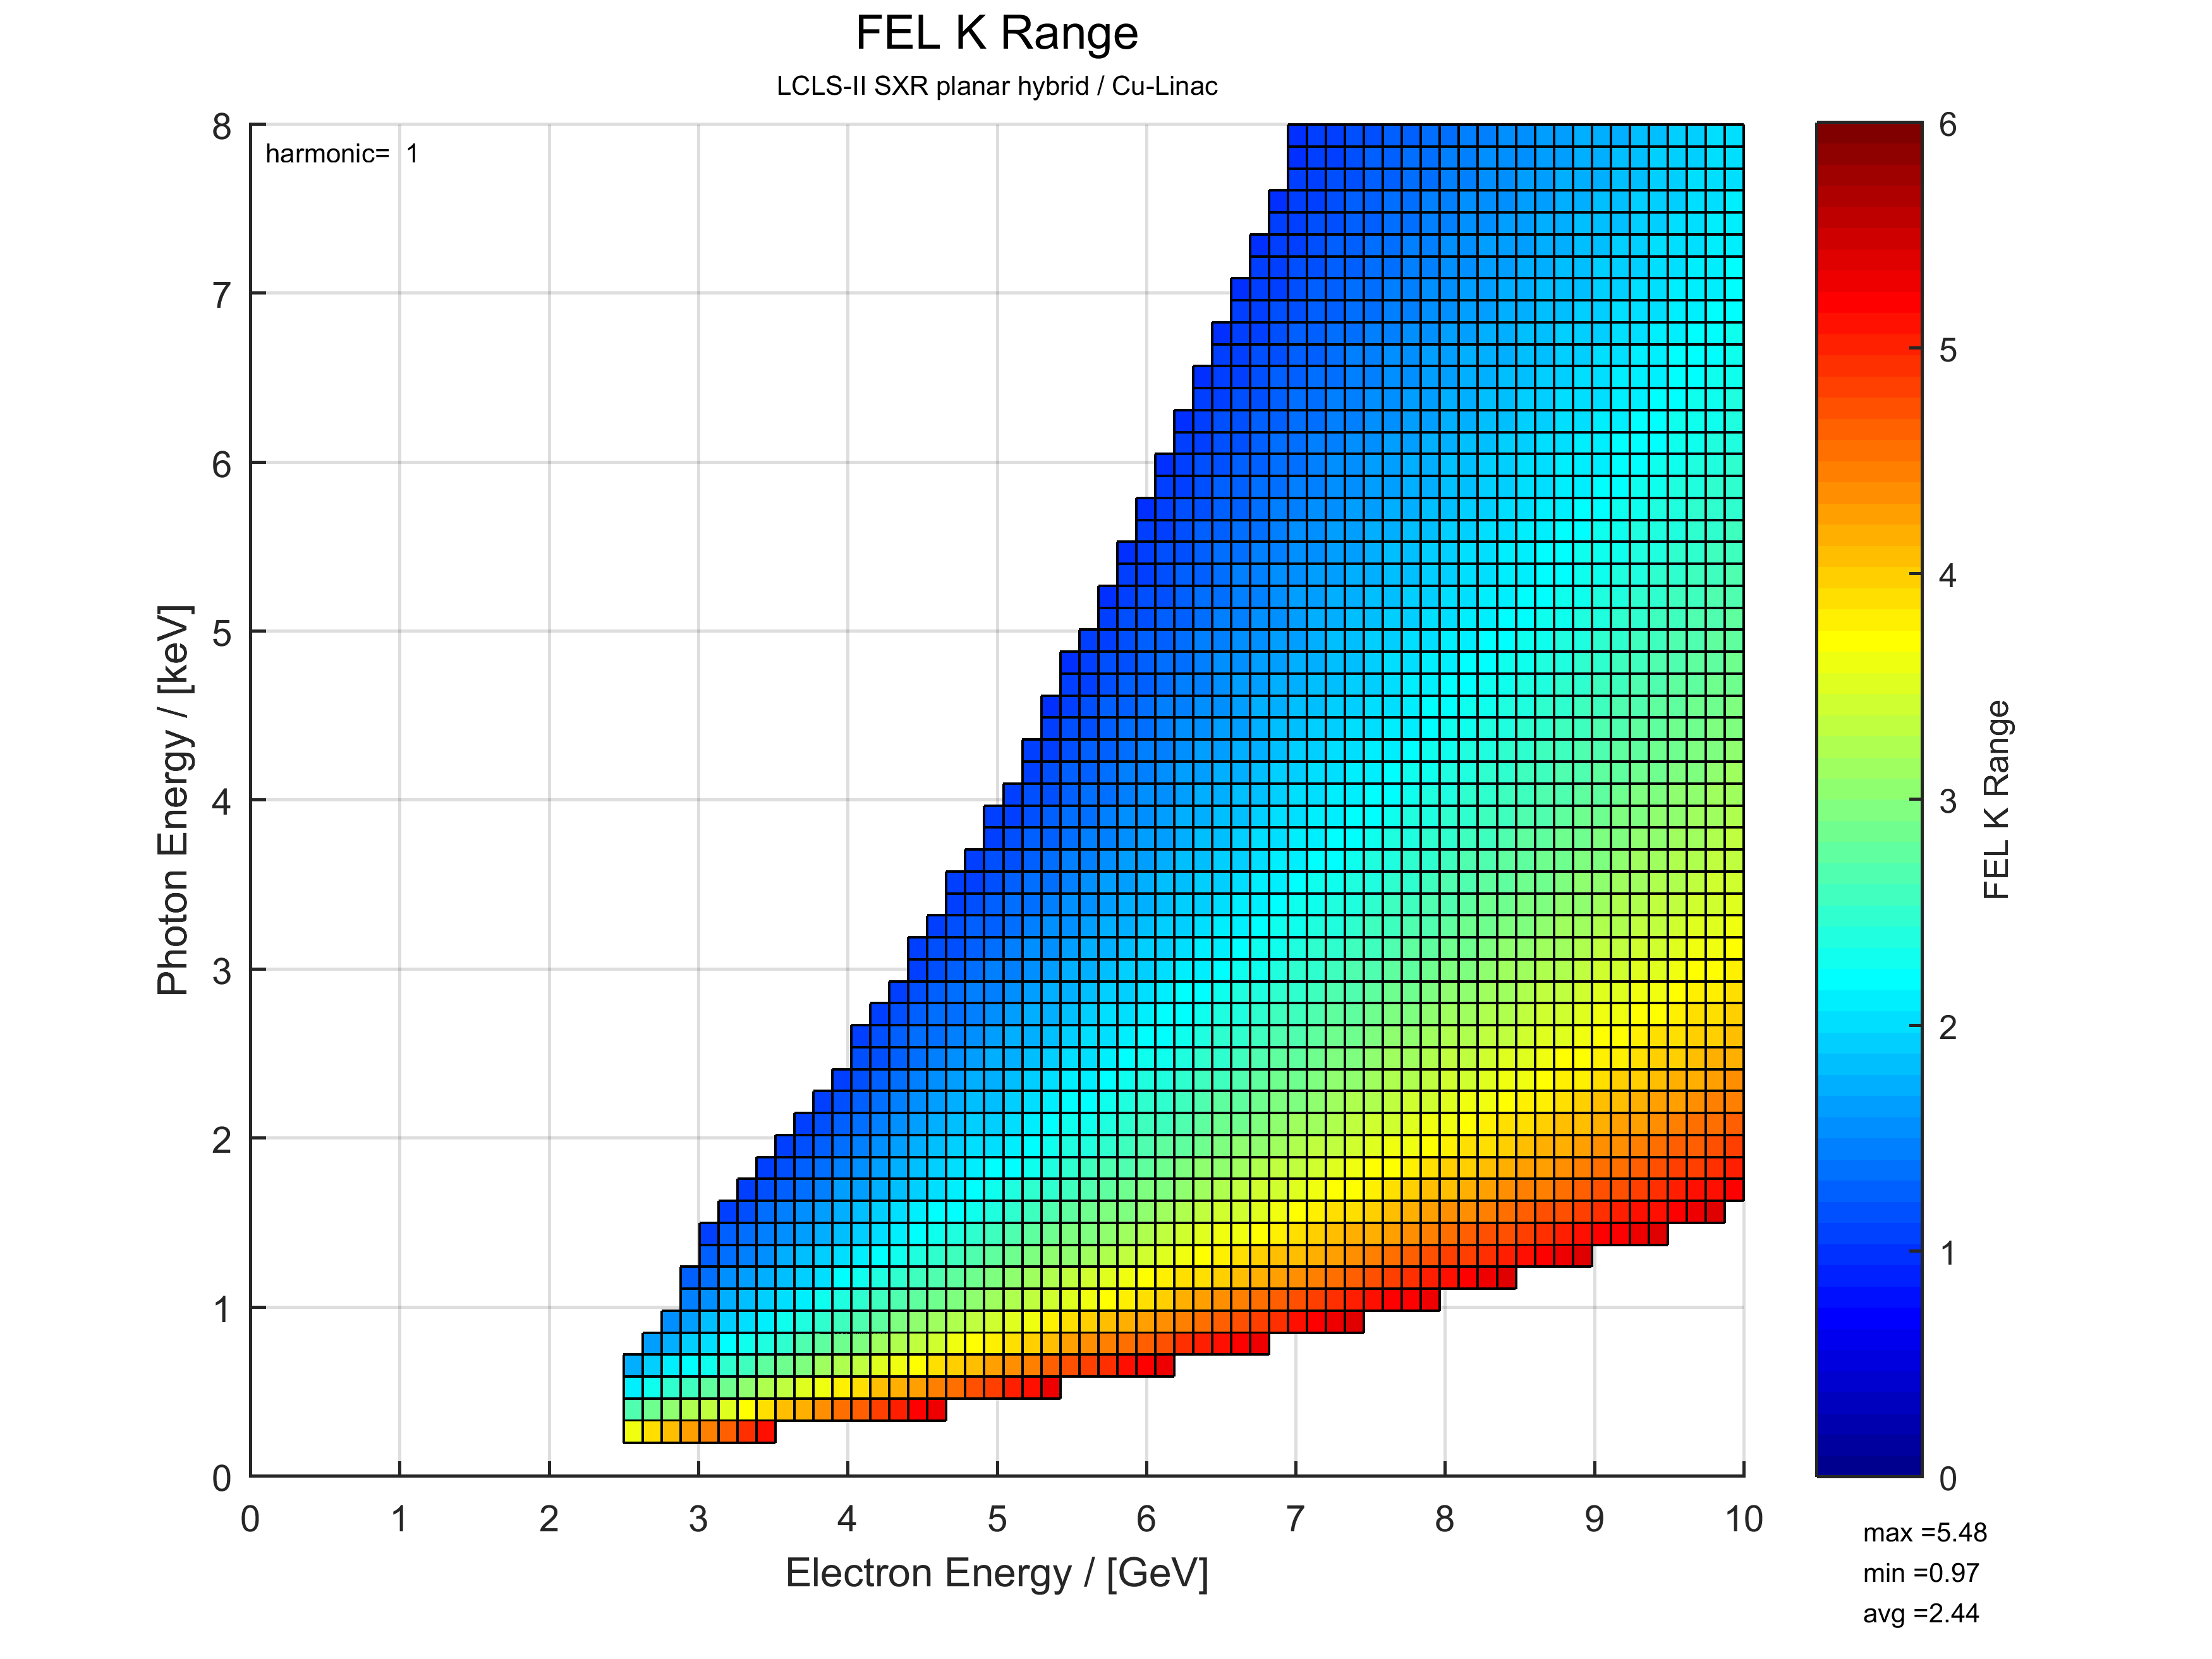
\includegraphics[width=\linewidth]{CuL_SXR_HorzPolPlanHybrid_K.eps}
	\includegraphics[width=\linewidth]{HeinzDieter_lcls2_SXU_range_lcls-tn-18-4.rangeFig.eps}
	}
\vspace{-1\baselineskip}
\caption{\label{fig::sxu_K} Soft x-ray undulator tuning range. \cite{HeinzDieter_SXU_twocolor}
	}
\end{wrapfigure}

The inference model will be trained based on a transfer learning paradigm whereby the central hidden layers, e.g. the simulation trained layers, will be optimized to recover x-ray pulse shapes given simulated angular streaking results.
The next step of the model training then adds a thin surface set of layers at the input side that is connected to the raw data of the detector.
We expect that such an architecture will preserve the physics of angular streaking as contained in the simulations, while also incorporating the raw sensor calibrations as well as adjusting to any remaining systematic errors in the retrieval interpretation.
By performing different algorithms on the same data, we can benchmark the pre-analysis that will ultimately be used to enhance resolution in the retrieval while maintaining the very high throughput needed for real-time analysis.

This chain of analysis will be compiled for FPGA deployment.  
By deploying to FPGA, we will only need to transfer the reconstructed x-ray pulse description rather than each of the individual raw waveforms. 
We will leverage our close collaboration with the Stanford CS/EE group of Kunle Olukotun, in particular though a shared Graduate Student Fellow, to deploy the analysis chain to FPGA as a very high throughput ($10^6$ Fps) and low latency ($\sim10~\mu$s) streaming inference engine.

